% ----------------------------------------------------------
% Consciousness subsection
% ----------------------------------------------------------
\subsection{Consciousness}
A logical moment can be formed by a division (first moment) or by logical subdivisions (other moments).
	\begin{figure}[H]
	\caption{Logical interval}
	\label{fig:consciousness_logical_moments}
	\centering
	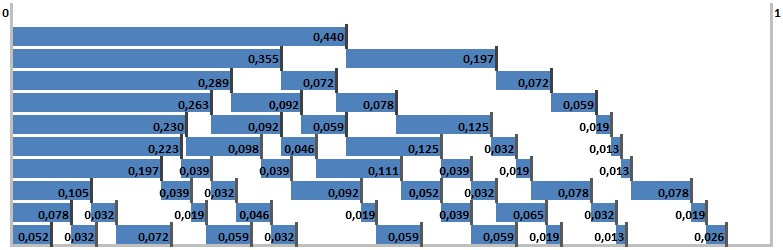
\includegraphics[scale=.7]{sections/images/consciousness_logical_moments.jpg}
	\floatfoot{Example of a logical interval with ten logical moments.}%\footnotemark}
	\end{figure}
	%\footnotetext{Fonte: note}

Consciousness is the logical moments of an expansion represented in its units.
	\begin{figure}[H]
	\caption{Conscious logical interval}
	\label{fig:consciousness}
	\centering
	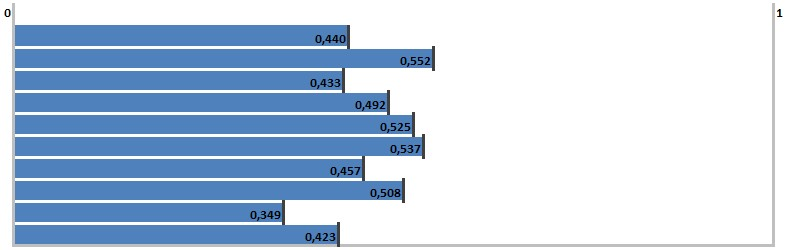
\includegraphics[scale=.7]{sections/images/consciousness.jpg}
	\floatfoot{Example of a conscious logical interval with ten units of logical moments.}%\footnotemark}
	\end{figure}
	%\footnotetext{Fonte: note}

It can be seen in Table \ref{tab:10000_all} that the probability of 99.99\% of the samples in a population (Range), which increase in quantity as the logical moments increase, tends to be increasingly in the center of the logical interval and this centralization tends to infinity.
	\begin{figure}[H]
	\caption{Centralization of 99.99\% of the samples}
	\label{fig:centering_of_99_range}
	\centering
	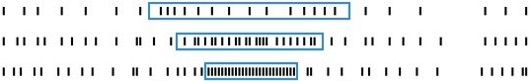
\includegraphics[scale=1]{sections/images/centering_of_99_range.jpg}
	\floatfoot{Tendency to center the range of 99.99\% of the samples.}%\footnotemark}
	\end{figure}
	%\footnotetext{Fonte: note}

Consciousness tends toward the representation of a logical wave, the largest logical wave in a population (a histogram of the normal distribution) as shown in the figure \ref{fig:trend_chart_of_normal_distribution}. All of the aspects listed below are inherent in the logical abstraction called consciousness.

\subsubsection{Infinite}
One of the most important aspects that the negation of nothingness brings (negation of self), is infinity, that is, in any logical interval the infinite fits again. The primordial logic that started the entire logical interval is the same found in its subsequent intervals (subintervals). This substantiates how a high-level logic like the human subconscious explains primordial logic, since it is not necessary to go back to the first logical moment of the interval to deduce it, as this phenomenon is omnipresent throughout the interval.

\subsubsection{Waves}
Probabilistically, the distribution of new samples from a population tends to concentrate more samples toward the median of the population as the frequency of samples increases in this direction. However, the distribution of these samples with uniform growth frequencies is infinitesimal compared to the random possibilities of this growth. Thus, the tendency of these growth frequencies toward the median, together with the very low (infinitesimal) probability of this growth being uniform, leads to frequencies in the waveform. The relationship of the density or amplitude of a wave to its length is detailed in the next subsection.
	\begin{figure}[H]
	\caption{Waveform}
	\label{fig:consciousness_waves}
	\centering
	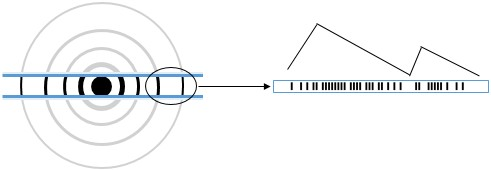
\includegraphics[scale=.8]{sections/images/consciousness_waves.jpg}
	\floatfoot{Wave pattern inferred by the trend of this distribution with higher frequencies towards the population median and very low probability of uniform growth of these frequencies.}%\footnotemark}
	\end{figure}
	%\footnotetext{Fonte: note}

Merging one wave into another eliminates its discrepancy and makes that wave cease to exist and become part of the first wave, which has its peak closer to the median, in this example. A wave doesn't die, it just merges with another wave closer to it.
	\begin{figure}[H]
	\caption{Wave unification}
	\label{fig:consciousness_uniform_wave}
	\centering
	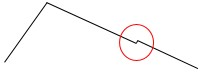
\includegraphics[scale=1]{sections/images/consciousness_uniform_wave.jpg}
	\floatfoot{Waves being unified to exemplify the uniform growth of the samples.}%\footnotemark}
	\end{figure}
	%\footnotetext{Fonte: note}

\subsubsubsection{Wavelength and amplitude}
The histogram is used in the figures in this subsection and later to facilitate visualization and understanding of the distribution of samples in a population, because it represents very well the density curves of a population, according to the different views of the Figure \ref{fig:consciousness_wave_histogram}, representing only one interval or wavelength paired by the median of the population.  
	\begin{figure}[H]
	\caption{Histogram in different views}
	\label{fig:consciousness_wave_histogram}
	\centering
	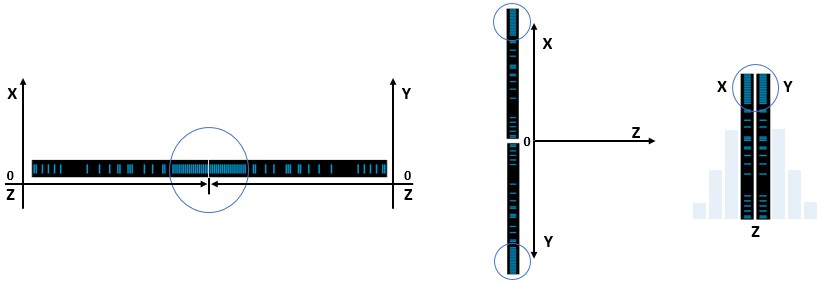
\includegraphics[scale=.7]{sections/images/consciousness_wave_histogram.jpg}
	\floatfoot{Different ways of population representation in a histogram.}%\footnotemark}
	\end{figure}
	%\footnotetext{Fonte: note}}
The length and amplitude of waves establish a quantity-per-interval or unit relationship. These units are established by wave entanglement, as seen in the next subsection. Thus, amplitude is the density of a wavelength, the density of some interval.  

When adding a new sample to the population, the entire interval is proportionally distributed to match that sample. When looking at the population at smaller intervals or wavelengths, their wave amplitudes will conform to the distribution of samples from these subintervals proportionally, as shown in Figure \ref{fig:consciousness_space_volume_amplitude}.
	\begin{figure}[H]
	\caption{Wavelength vs. Amplitude}
	\label{fig:consciousness_space_volume_amplitude}
	\centering
	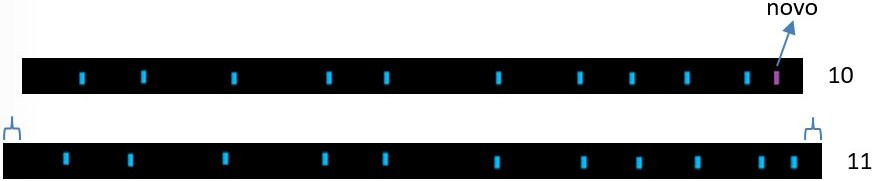
\includegraphics[scale=.4]{sections/images/consciousness_space_volume_amplitude.jpg}
	\floatfoot{Relationship of wave length and amplitude.}%\footnotemark}
	\end{figure}
	%\footnotetext{Fonte: note}}
	
Another important factor is that new samples tend to be more distributed at the peak of the interval, probably the densest place in the wave. In Figure \ref{fig:consciousness_space_amplitude_growth} the peak is represented in the upper part of the subinterval that makes up the peak of the wave (because it is the densest interval that makes up the peak and because the upper part of the interval is closer to the population median) . However, the peak can be at any other point in the subintervals that make up the peak of a wave.
	\begin{figure}[H]
	\caption{Wave amplitude - peak}
	\label{fig:consciousness_space_amplitude_growth}
	\centering
	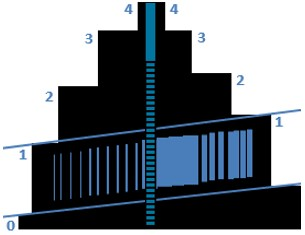
\includegraphics[scale=.6]{sections/images/consciousness_space_amplitude_growth.jpg}
	\floatfoot{Trend of the highest concentration of samples in the subintervals of a wave.}%\footnotemark}
	\end{figure}
	%\footnotetext{Fonte: note}}

In large intervals with many logical moments a smaller discrepancy of wave amplitudes is observed. In such intervals large systems of objects can be observed. The larger the intervals, the more balanced they grow towards the population median (probabilistically) as seen in Figure \ref{fig:consciousness_space_subconsciousness}. The lowest wave (dark blue) is the base wave of the system, that is, the wave that formed the other waves. Wave systems can be complex, having several nested waves. More complex intervals with this feature can represent, for example, the universe, then galaxies, stars, planets, etc.
	\begin{figure}[H]
	\caption{Wave amplitude at large intervals or lengths}
	\label{fig:consciousness_space_subconsciousness}
	\centering
	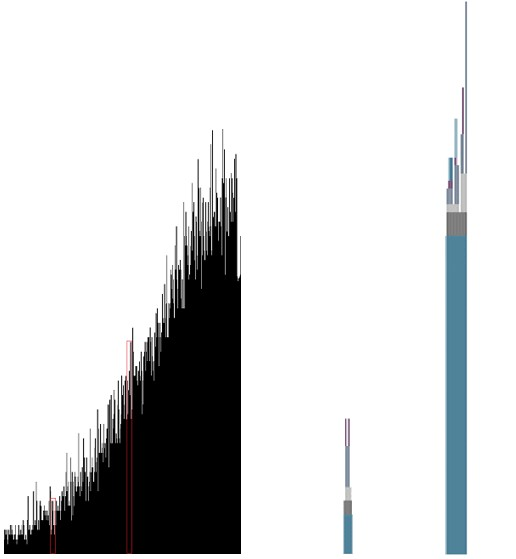
\includegraphics[scale=.45]{sections/images/consciousness_space_subconsciousness.jpg}
	\floatfoot{Smaller wave discrepancy at large intervals.}%\footnotemark}
	\end{figure}
	%\footnotetext{Fonte: note}

In smaller intervals and with many logical moments a greater discrepancy in wave amplitudes is observed. In these intervals smaller object systems can be observed. The smaller the intervals are, the more unbalanced they will grow towards the population median (probabilistically) as seen in the figure \ref{fig:consciousness_space_subconsciousness_min}. The lowest wave (dark blue) is the base wave of the system, that is, the wave that forms other waves. More complex wave systems with this feature can represent, for example, the atom, which is very small, present in huge quantities, and the particles orbiting its nucleus (electrons) are much more distant from it.
	\begin{figure}[H]
	\caption{Wave amplitude at small intervals or lengths}
	\label{fig:consciousness_space_subconsciousness_min}
	\centering
	
\includegraphics[scale=.45]{sections/images/consciousness_space_subconsciousness_min.jpg}
	\floatfoot{High wave discrepancy at small intervals.}%\footnotemark}
	\end{figure}
	%\footnotetext{Fonte: note}}

\subsubsubsection{Entanglement}
The most similar samples in terms of frequency and distribution are the samples that are part of the same wave. They are non-overlapping, opposite frequencies that complete each other.

Probabilistically, the two complementary parts of a wave tend to be at approximately equal distances, equidistant from the median, but this is not a rule and the complementary parts of a wave may be at different distances from the median. The phenomenon of parity of the parts of a wave is called wave entanglement.

These pairs tend to be formed by probability, where equal wavelengths have the same probability of samples distribution at two or more different points in the population. 

Intervals with similar temporal frequencies and spatial distributions are intervals formed by the same probabilistic unit, that is, intervals that have the same probabilistic scenario or context at a given logical moment. Being in the same probabilistic scenario (probabilistic units), these intervals have their samples in the same space-time scenario, which is called space-time lattice and is formed by the largest probabilistic unit in the population (all the samples in the population intermediated by the median). 

These entanglements form smaller waves (subconsciousnesses), similar to the largest wave in the entire interval, usually entangled by the population median (consciousness). Consciousness is the logic of the entire interval, while it forms subconsciousnesses or sublogics, like small waves of a larger wave.These small waves are similar to the pattern of the larger wave.  Thus, a change in the larger wave (consciousness) are also changes in the smaller waves (subconsciousnesses) - a change that is induced indirectly by subconsciousnesses, analogous to the compression of gas in a cylinder, where by adding a new molecule of gas in the partially filled cylinder, closer or tighter these molecules will be inside it.  The opposite is also true, a new sample in a subconsciousness that is directly observed by it is also a change of the consciousness and will be induced indirectly by other subconsciousnesses, as shown in the Figure \ref{fig:consciousness_space_plan}.
	\begin{figure}[H]
	\caption{Subconsciousness}
	\label{fig:consciousness_subconscious}
	\centering
	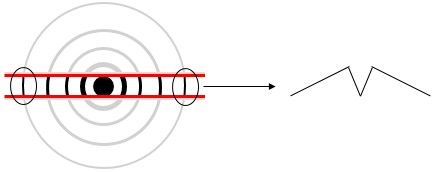
\includegraphics[scale=.8]{sections/images/consciousness_subconscious.jpg}
	\floatfoot{The wave pattern forms subconsciousnesses similar to the pattern created by consciousness, as seen in Figure \ref{fig:trend_chart_of_normal_distribution}.}%\footnotemark}
	\end{figure}
	%\footnotetext{Fonte: note}
	
The entanglement of waves can occur at different levels or intervals, as seen in Figure \ref{fig:consciousness_subconscious_entanglement}, which forms nested wave systems. The borderless braces (right) identify the intervals at which a new sample triggered the jump, as seen in the next subsection. The numbered arcs indicate the order of the entanglements. An entanglement can occur equidistantly from the median without the jump, like the first entanglement (violet).

The largest entanglement is shown in the examples in Figure \ref{fig:consciousness_subconscious_entanglement} as the first entanglement (violet), which occurred when that interval was the smallest, probably.  Large intervals tend to be kept ordered by the reordering of their subintervals subsequently. The largest wave is commonly entangled by the population median.

The smaller intervals tend to get the entanglement first, and these reorderings caused by them allow the entanglement of pairs with larger intervals. Entangled pairs are the two opposite sides of a wave (peak or valley) and are entangled by its median, which may coincide with the population median when it is the largest probabilistic wave of the entire interval.
	\begin{figure}[H]
	\caption{Wave entanglement levels - wavelengths}
	\label{fig:consciousness_subconscious_entanglement}
	\centering
	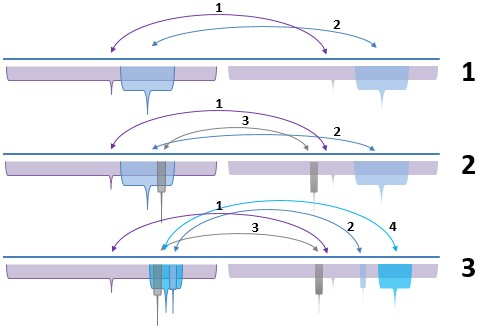
\includegraphics[scale=.8]{sections/images/consciousness_subconscious_entanglement.jpg}
	\floatfoot{Examples of entanglement levels of waves or levels of wavelengths.}%\footnotemark}
	\end{figure}
	%\footnotetext{Fonte: note}

The possible wavelengths of a population are defined by these levels of wave entanglement. Thus, regardless of the order of the jumps, larger entanglements are the longer wavelengths and smaller entanglements are the shorter wavelengths, which allows larger waves to have smaller subwaves. 

Every entanglement is a wave and the meeting of two entanglements does not lead to a new entanglement, only the sum of these waves, because they are already entangled.

The entanglement occurs in very small intervals. Once entangled, each new sample can cause movement, depending on the more or less rarefied environment. Larger intervals are formed by adding smaller intervals already entangled through movement and by adding new samples.

\subsubsubsection{Jump}
The jump is a reordering done by wave entanglement, as the samples of the entangled pairs are no longer equivalent with the addition of new samples from one side of the pair. The jump occurs on one side of a pair of waves and is a reordering.

In Figure \ref{fig:consciousness_space_subconscious_observation_jump} the entanglement of waves (represented by columns of a histogram to facilitate the visualization of the interval) is observed. The reordering made by the entanglement causes a jump in the coordinates (X, Y and Z) according to the Space subsection.
	\begin{figure}[H]
	\caption{Reordering - jump}
	\label{fig:consciousness_space_subconscious_observation_jump}
	\centering
	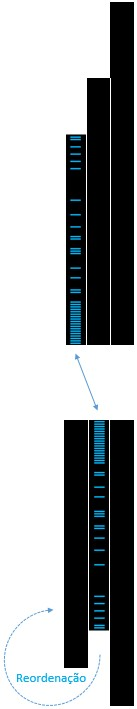
\includegraphics[scale=.53]{sections/images/consciousness_space_subconscious_observation_jump.jpg}
	\floatfoot{Jump caused by non-equivalence of the entangled pair with the addition of new samples on one of its sides.}%\footnotemark}
	\end{figure}
	%\footnotetext{Fonte: note}

As an example, a photon entering the electron's interval can unbalance one side of the electron's entangled pair, which makes it jump, but since the electron's interval is small and the photon is fast (because it is even smaller) it quickly leaves the electron's interval, which becomes unbalanced again and returns to the energy level equivalent to the one before the jump.

\subsubsection{Time}
Time is the addition of new logical moments between existing moments as the self-negation of primordial logic proceeds. The changes are cumulative and as the number of logical moments increases, the less relevant each new moment within the conscious interval will be. One in a hundred is more relevant than one in a thousand. 
	\begin{figure}[H]
	\caption{Time}
	\label{fig:consciousness_time}
	\centering
	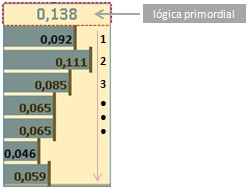
\includegraphics[scale=.8]{sections/images/consciousness_time.jpg}
	\floatfoot{Progression of time as logical moments advance.}%\footnotemark}
	\end{figure}
	%\footnotetext{Fonte: note}

In the introduction to this paper it was presented that primordial logic is a sequence of negations of itself at time zero, that is, at no time between its negations does logic [being], guaranteeing the primordial premise of the logical constant, [NOT BEING]. Thus, logic is an infinite, simultaneous and generalized sequence, a constant. In the observer-driven experience of time, the ordering of each sequence is the essence of this logical quantity and therefore more relevant than its origin, which is of a simultaneous nature, transcending time.

Each population has a different order in its sequence and it is this order that gives rise to the logical quantity called time. It is this order of the universe or of consciousness that will give the notion of what happens before or after, that is, the past, the present and the probabilistic future prospections.

Another important factor when observing time (the observer is more detailed in the consciousness subsection – Observer and life) is that, probabilistically, subconsciousnesses or intervals closer to the population median will have a larger addition of new samples in their intervals, which are directly observed by these subconsciousnesses. On the other hand, subconsciousnesses far from the population median will have a smaller addition of samples in their intervals and are subject to a larger number of indirectly induced changes, as shown in Figure \ref{fig:consciousness_subconscious}.  This phenomenon of temporal observation provided by the probability of the population distribution avoids the twin paradox \cite{twin_paradox}.

Prospections of the observer's future are based on the probabilistic distribution of the population and, therefore, on the probabilistic distribution of each sub-interval of the population. The universe tends to be probabilistic, while random at levels of detail (which makes events different), yet predictable at some level, as shown in Figures \ref{fig:consciousness_logical_moments} and \ref{fig:consciousness}. 

\subsubsection{Space}
In Figure \ref{fig:consciousness_space_waves}, the sample density of a population is shown, where pairs tending to the same probabilistic distribution are placed side by side and represented in histogram form. The formation of these pairs comes from wave entanglement.
	\begin{figure}[H]
	\caption{Entangled pairs represented in three spatial dimensions}
	\label{fig:consciousness_space_waves}
	\centering
	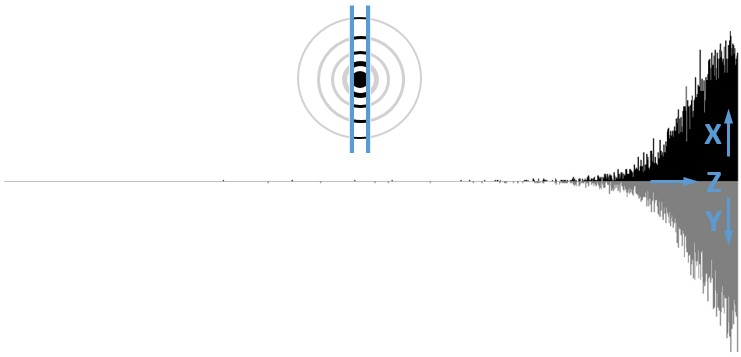
\includegraphics[scale=.7]{sections/images/consciousness_space_waves.jpg}
	\floatfoot{Example of entangled waves, represented in histogram form and obtained by the Logic\_WavePattern algorithm. \footnotemark}
	\end{figure}
	\footnotetext{The Logic\_WavePattern algorithm can be seen in Appendix \ref{app:algorithms}.}

The area grows quadratically to the increase in the amplitude of a wave (columns of the histogram), since the jump caused by the entanglement of the waves and the probabilistic distribution of samples in the interval naturally tend to maintain an equivalent growth in the pairs that form a wave. This aspect configures the inverse square law, which will be further explored in the subsection of Gravitational force.

By plotting the spatial dimensions of the graph of Figure \ref{fig:consciousness_space_waves} on a 3D distribution graph and distributing their endpoints (neglecting their volumes and possible internal points), something like a spiral is obtained (like eddies in water or air), even on very small data volumes (few logical moments), as in Figures \ref{fig:consciousness_space_3DScatter15000-10} and \ref{fig:consciousness_space_3DScatter_200000-2}. The points tend to move in a spiral shape approximately, as shown in the next subsection.
	\begin{figure}[H]
	\centering
		\begin{subfigure}[H]{0.47\linewidth}
		\centering
		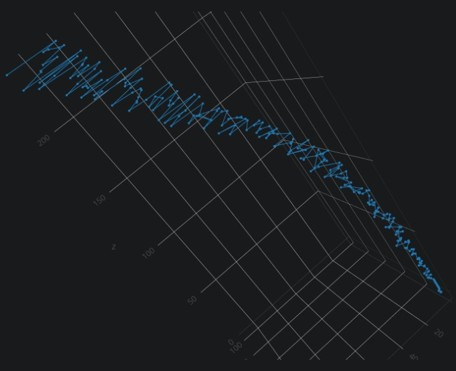
\includegraphics[width=1\linewidth]{sections/images/consciousness_space_3DScatter15000-10.jpg}
		\caption{15,000 samples or moments}
		\label{fig:consciousness_space_3DScatter15000-10}
		\end{subfigure}
	
		\begin{subfigure}[H]{0.47\linewidth}
		\centering
		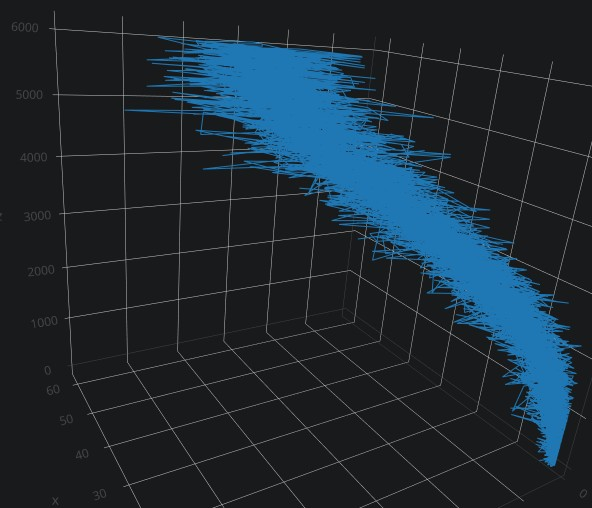
\includegraphics[width=1\linewidth]{sections/images/consciousness_space_3DScatter_200000-2.jpg}
		\caption{200,000 samples or moments}
		\label{fig:consciousness_space_3DScatter_200000-2}
		\end{subfigure}%
	\caption{3D scatter plots generated with points similar to Figure \ref{fig:consciousness_space_waves}}
	\floatfoot{The histogram on the wave pattern and the data for generating the 3D scatter plots can be obtained by running the Logic\_WavePattern algorithm. \protect\footnotemark}
	\end{figure}
	\footnotetext{The Logic\_WavePattern algorithm can be seen in Appendix \ref{app:algorithms} and the 3D scatter plots can be accessed at: \url{https://chart-studio.plot.ly/create/?fid=ren.stuchi:5&fid=ren.stuchi:4} e \url{https://chart-studio.plot.ly/create/?fid=ren.stuchi:7&fid=ren.stuchi:6}}

Probabilistically, the high concentration of samples in a population is at its peak, towards the median of the population. Thus, due to the probabilistically high concentrations of samples in smaller and smaller intervals of a wave, the peak will occupy a smaller and smaller proportional subinterval within the population, as seen in Figure \ref{fig:consciousness_flat_universe}. The figure \ref{fig:total_comparison_chart_with_99_range} is based on Table \ref{tab:10000_all} and also demonstrates this feature, that within the population it can show an approximately homogeneous and flat universe in its distribution even though its samples tend to the reference line.  
	\begin{figure}[H]
	\caption{Flat universe}
	\label{fig:consciousness_flat_universe}
	\centering
	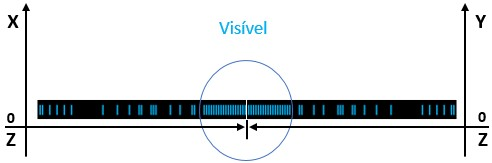
\includegraphics[scale=.4]{sections/images/consciousness_flat_universe.jpg}
	\floatfoot{Concentration of 99\% of samples.}%\footnotemark}
	\end{figure}
	%\footnotetext{Fonte: note}

\textbf{Obviously the representation and motions of the interval or its entangled subintervals cannot be faithfully represented in 1 or 2 dimensions, as entanglement is inherent (inseparable) essence of 3 dimensions.}

Each new sample is time and also space (movement or change). Each new sample added within a subinterval will cause it to move according to the distribution of its new samples. The interval or its subintervals can move in any direction, but just as in a 1D distribution (Z-axis of Figure \ref{fig:consciousness_space_plan}) the samples are concentrated in the highest value part of the plane, in 2D or 3D is analogous and the same occurs, as shown in the subinterval of Figure \ref{fig:consciousness_space_plan}. Both the interval and the subintervals have their highest sample concentrations towards their inner reference line and the reference lines of their upper intervals. This makes something approximating a histogram representation come naturally. The interval and its subintervals have their sizes in X, Y and Z proportional to their sizes within the population in 1D representation (Z-axis of Figure \ref{fig:consciousness_space_plan}), so their internal scales are related to the number of samples that they have.
	\begin{figure}[H]
	\caption{Spatial distribution and movement}
	\label{fig:consciousness_space_plan}
	\centering
	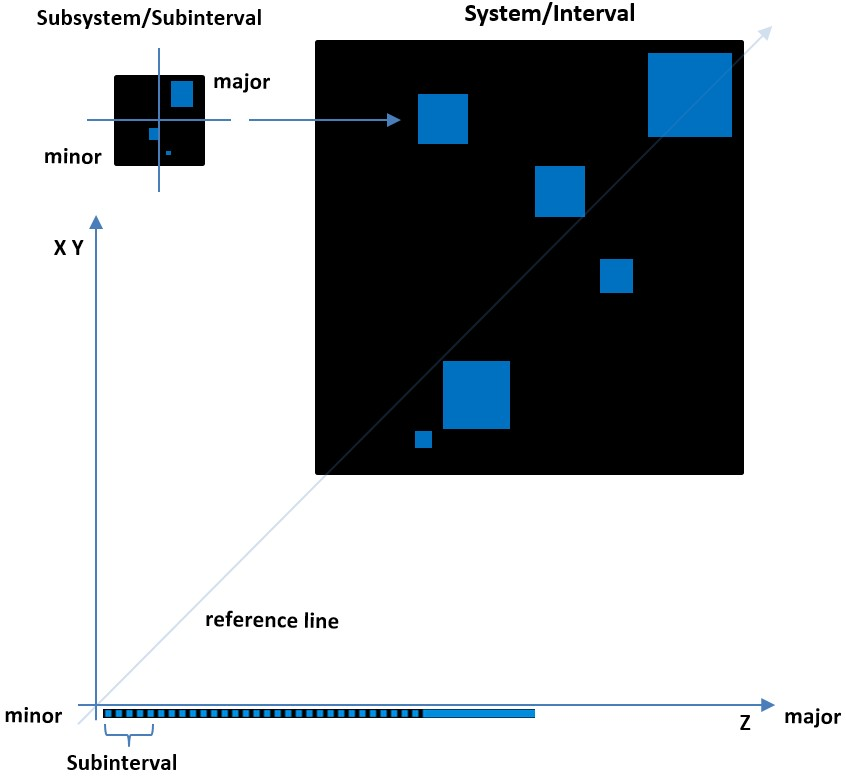
\includegraphics[scale=.6]{sections/images/consciousness_space_plan.jpg}
	\floatfoot{Spatial distribution and movement of subintervals and population interval.}%\footnotemark}
	\end{figure}
	%\footnotetext{Fonte: note}

A new sample in a subinterval moves this and its upper intervals, because a change in a subinterval is also a change in its upper intervals. The movement is continuous and its time and space scales are relative to the basic unit of the population (1 sample [space] to each new sample from the population [time]). For example, a subinterval may be moving in one direction at 2 samples (space) at each new sample of the population (time) and will continue in this motion until it receives two opposing internal samples or collides with some sample in its motion, in more or less rarefied environments, that slows it down or causes it to stop (laws of dynamics).

The entanglement occurs in very small intervals and they form at the base of their upper intervals, according to the Z-axis. Once entangled, each new sample can cause movement, depending on the more or less rarefied environment. Larger intervals are formed by adding smaller intervals already entangled through movement and by adding new samples, as per the Entanglement subsection. Thus the movement of electrons within the atom is not totally continuous, because the jumps cause new entanglements that redefine their positions, configuring layers.

A subinterval can naturally leave the gravitation of its upper interval. This occurs most easily with very small and fast intervals (many samples concentrated in a small interval - peak) favored by their movement in a rarefied environment due to their size.

It is very difficult to know the position of the interval or a subinterval by looking at a 1D representation, because each new sample moves the subinterval and the interval and this interaction requires a calculation for representation that would take until a naturally 3D representation again.

Each subinterval when it is entangled arises at the bottom of its upper interval. Then adding new samples into this subinterval that has just emerged will cause it to move up into its upper interval, and this is the direction of all entanglements that do not have subintervals, to move up as they add samples and speed toward the reference line. But the environment may not be rarefied which makes this movement difficult (and may keep it stationary depending on how dense that environment is). Thus, in Figure \ref{fig:consciousness_space_plan_nosubinterval} an interval that does not yet contain subintervals is displayed, so it moves up and gains speed with each new sample it receives, and its rise will either be centralized if its samples are evenly distributed or with a centralized peak, or it will be skewed to the right or left as the highest concentration of samples is more on one side than the other (it is more common for the concentration of samples to be toward the population median).
	\begin{figure}[H]
	\caption{ Interval without subintervals}
	\label{fig:consciousness_space_plan_nosubinterval}
	\centering
	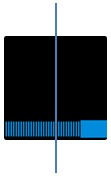
\includegraphics[scale=.7]{sections/images/consciousness_space_plan_nosubinterval.jpg}
	\floatfoot{ Moving an interval without subintervals.}%\footnotemark}
	\end{figure}
	%\footnotetext{Fonte: note}
	
Intervals that have subintervals can move in any direction, since their subintervals can receive jumps and through these new entanglements the position of these subintervals are reset to the base of their upper interval and thus this interval can have a destruction of subintervals in any direction, whether they are denser or less dense, as the subinterval in Figure \ref{fig:consciousness_space_plan}.

\subsubsubsection{Spiral}
As the X, Y, and Z coordinates of the entangled pairs of a population tend to increase, their arrangement in a three-dimensional coordinate system will follow a diagonal reference between these three axes, as shown in Figure \ref{fig:consciousness_space_spiral_reference_line}. The observed spiral pattern does not invalidate other possible movements in space. Often, it is not possible to immediately observe the spiral pattern in the movements of an interval (subinterval), yet this pattern underlies many of these movements.  Taking human movements, for example, there are predominant cycles of going and coming home, going to and from work, waking up and sleeping, that is, habits are similar to movements in cycles (spiral movements).
	\begin{figure}[H]
	\caption{Three-dimensional coordinate system}
	\label{fig:consciousness_space_spiral_reference_line}
	\centering
	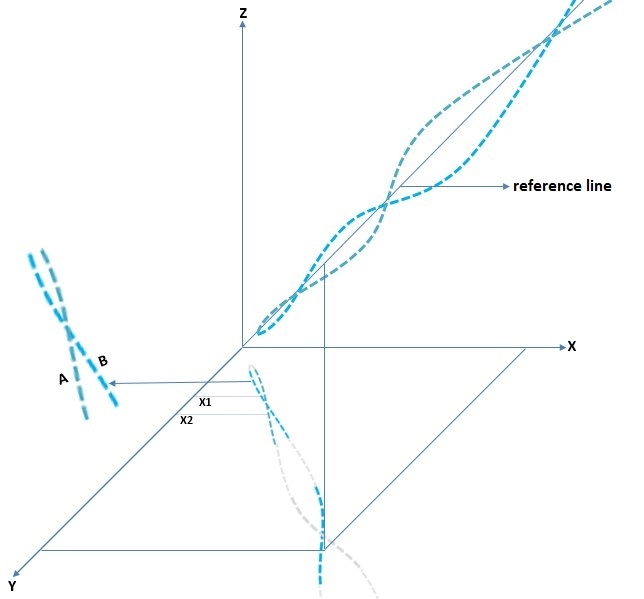
\includegraphics[scale=.7]{sections/images/consciousness_space_spiral_reference_line.jpg}
	\floatfoot{Probabilistic reference line for distribution of a population in a three-dimensional plane.}%\footnotemark}
	\end{figure}
	%\footnotetext{Fonte: note}}

In Figure \ref{fig:consciousness_space_spiral_reference_line} points X1 and X2 can also be observed. These points were mirrored in the X and Y coordinates to make it easier to observe that raising the Z axis also raises the X or Y axis, regardless of their minimum probabilistic points. The dashed lines show the most probable paths to the A and B intervals. Thus, when a part of the interval is at its maximum midpoint (X and/or Y axes) the probabilistic tendency is that it receives fewer samples than the part of the interval that is at its minimum midpoint. This spiral effect is more noticeable the larger an interval and its quantity of samples, as the more probable and stable these paths will be.

The continuous motion in a rarefied environment also helps in the formation and maintenance of the spirals. As the samples are added to the subintervals their velocities increase towards the reference line, and because this addition is not uniform (varying between peaks and valleys) and the motion is approximately continuous the subintervals can drift or slide from one side of the reference line to the other.

Each interval or subinterval (wavelength) has its own reference line. Just as within a meter there are centimeters, millimeters, etc., within an interval and subinterval there can be numerous other subintervals.
	\begin{figure}[H]
	\caption{Intervals and reference lines}
	\label{fig:consciousness_space_spiral_underlines}
	\centering
	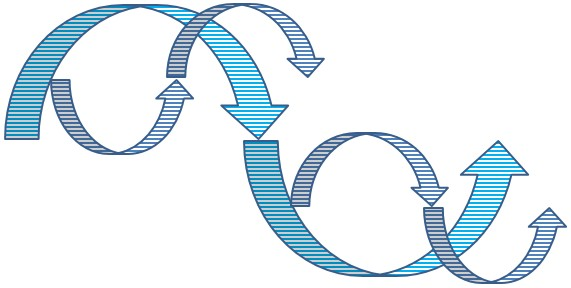
\includegraphics[scale=.5]{sections/images/consciousness_space_spiral_underlines.jpg}
	\floatfoot{Spirals at different intervals and their reference lines.}%\footnotemark}
	\end{figure}
	%\footnotetext{Fonte: note}}

\subsubsection{Fundamental forces}
The gravitational force, the electromagnetic force and the nuclear force correspond to the so-called fundamental forces of nature. These fundamental forces are not forces as such, but probabilistic aspects of population distribution and wave entanglement.

\subsubsubsection{Gravitational force}
The gravitational force is not a force itself, but an aspect of the probability of distributing new samples towards the population median, according to the central limit theorem. This probabilistic sense makes waves have a probable path to follow within the population, that is, the peak of population samples or the peak of the largest wave in the population. In the same way, they also make the samples within an interval have a probable path to follow, the peak of samples of the interval or the peak of the wave. These sample peaks are usually the most easily observable part of the sample interval since they occupy a not so small area.

In Figure \ref{fig:consciousness_gravitational_force} it can be seen that the most easily observable part is slightly to the right at the peak of the wave. This wave tends to move up and to the right, in a diagonal direction to the peak of its upper interval. It can also be seen in this figure that it has a slightly higher density of samples on the right, and these samples are more evenly distributed. This density and uniformity indicates the probabilistic path this interval is traveling and its speed in that direction (the higher this density and uniformity).
	\begin{figure}[H]
	\caption{Gravitational force}
	\label{fig:consciousness_gravitational_force}
	\centering
	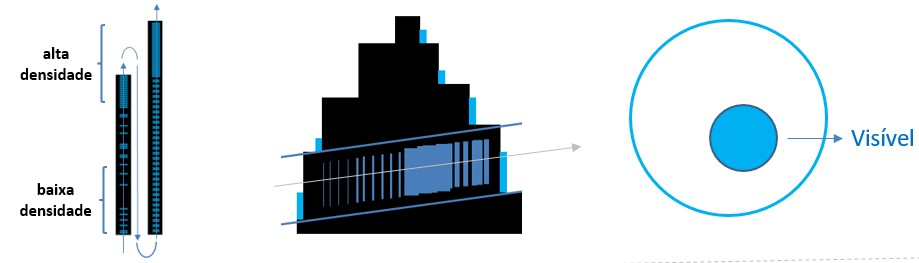
\includegraphics[scale=.7]{sections/images/consciousness_gravitational_force.jpg}
	\floatfoot{Gravitational aspect - the probabilistic direction of the distribution of new samples within an interval.}%\footnotemark}
	\end{figure}
	%\footnotetext{Fonte: note}

As seen in the Wavelength and amplitude subsection, the area of an interval grows quadratically, since the jump caused by the entanglement of the waves and the probability distribution of the samples tends to maintain an equivalent growth in the pairs that form a wave. This aspect configures the inverse square law, where, in the case of gravity, the closer the objects, the greater the probabilistic chances of new samples of the smaller object heading towards the larger object (since the larger object tends to be the peak of wave - the probabilistic direction within the wave). Thus, for being within a smaller square area and, consequently, having less possibility of movement, it ends up increasing the chances of these objects approaching with a much smaller amount of logical moments. On the other hand, the more distant the objects, the larger the area, the greater the positioning possibilities and the more logical moments are needed for the approach, featuring less attraction. Probability can also drive away more rarefied objects that should be further away from the denser and more easily observable part of a wave, as in the case of helium gas, for example. The distribution of new samples in the rarefied intervals is slower than in the denser intervals (otherwise they would not be rarefied), so these dense particles receive more samples in a shorter amount of time, occupying the front of the less dense particles.

\subsubsubsection{Electromagnetic force}
The electromagnetic force is not a force in itself, but an aspect of the entanglement of waves that intensifies at intervals or wavelengths with low entropy and with the spatial approximation (reduction of differences in the X, Y and Z axes) of these intervals.

Electromagnetism is related to intervals similar to the more uniform wave side found in Figure \ref{fig:consciousness_gravitational_force} (right), but with low entropy, that is, the same structure that facilitates the movement of objects added to the low entropy, which facilitates jumps. When intervals have low entropy, their approximation, either naturally through the structure that facilitates movement or through the distribution of new samples capable of creating this structure, such as electrification, makes the wave pairs of one interval very similar to the wave pairs of the other interval, which makes many of these pairs viable for wave entanglement to finding more ideal pairs in the other interval and vice versa. In this way, a rearrangement occurs between the intervals through wave entanglement, and this rearrangement makes these intervals more equalized (low entropy).

The blue lines in the figure \ref{fig:consciousness_electromaagnetic_force} show where the exchange of wave pairs by wave entanglement is most frequent, that is, where the waves are most probable to be similar. This is why magnets try to rotate to connect when they are face to face with the same pole. The gray line shows connections that occur in a much smaller number.
	\begin{figure}[H]
	\caption{Electromagnetic force}
	\label{fig:consciousness_electromaagnetic_force}
	\centering
	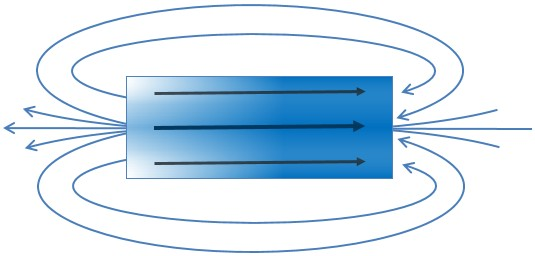
\includegraphics[scale=.7]{sections/images/consciousness_electromaagnetic_force.jpg}
	\floatfoot{Increased possibilities of wave entanglement due to probabilistic equalization in close and low entropy objects.}%\footnotemark}
	\end{figure}
	%\footnotetext{Fonte: note}

Figure \ref{fig:consciousness_electromaagnetic_force_entropy} shows an example of low entropy.
	\begin{figure}[H]
	\caption{Electromagnetic force - entropy}
	\label{fig:consciousness_electromaagnetic_force_entropy}
	\centering
	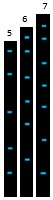
\includegraphics[scale=.9]{sections/images/consciousness_electromaagnetic_force_entropy.jpg}
	\floatfoot{Increased possibilities for wave entanglement due to low entropy.}%\footnotemark}
	\end{figure}
	%\footnotetext{Fonte: note}

The electromagnetic aspect is closely related to the low entropy of an interval and the possibility of entanglement of its pairs with surrounding pairs. The low entropy of an interval indicates that its samples are in some sort of order within it.

Probabilistically, the most similar wave pairs are found in the closest regions (blue lines in the figure \ref{fig:consciousness_electromaagnetic_force}). This occurs due to the growth of the number of samples towards the median of the population, however it is not a rule and the poles may reverse, that is, have more connections with the region of lower probability, even though most of the pairs that make up this region are increasing towards the median.

\subsubsubsection{Nuclear force}
The same probabilistic aspects that govern gravity and that can be seen in Figure \ref{fig:consciousness_gravitational_force} also govern the so-called nuclear forces. The difference is that in nuclear forces the intervals are smaller allowing a much larger amount of jumps and their waves are more discrepant, as shown in Figure \ref{fig:consciousness_space_subconsciousness_min}.

The strong and weak nuclear forces represent large concentrations of logic moments per population interval, a high density in a small interval. The large concentration of these samples is at the peak of the interval, which occupies a smaller and smaller subinterval within the wave (proportionately), due to the high concentration of samples in smaller and smaller intervals, as shown in Figure \ref{fig:total_comparison_chart_with_99_range}.

The penetration of these small and dense intervals by an excessive amount of logical moments (another similar interval), in a short period, causes the countless pairs of their subintervals to oscillate, potentiating the jumps. In this way the subintervals jump continuously, progressively and quickly until the probability distribution of the population normalizes the entire interval afterwards. Along with the jumps that will cause movements in large numbers of particles or intervals around them, there are a huge number of frictions at tremendous speeds caused by the collision of these small particles that cause great shock waves.

\subsubsection{Orbits}
The orbit definition can be defined in this study as the concept of spirals with the addition of the orientation of a probabilistic peak (gravity) instead of the reference line of the spirals, only.

Systems that orbit as described in the subsection on space (spiral - oriented by the reference line) are systems or intervals in which their peak is subdivided into subintervals and do not form a center of gravity, that is, all subintervals of the peak are not concentrated in one point of the system, thus orbiting the reference line of the interval. Probably galaxy clusters and superclusters are examples of this orbit. The spiral orbit (oriented by the reference line) is not restricted to large systems, this orbit is a feature that can happen in any size of interval.

Another type of orbit is defined when the subintervals that orbit the peak of the wave (which represents approximately 99.9\% of the samples in the interval) decrease their orbit speed as they move away from the peak. In Figure \ref{fig:consciousness_elliptical_orbit_system} the columns of the histogram in blue represent the peak of the wave. This decrease in velocity occurs gradually as these gray intervals move away from the peak of the wave, thus receiving a smaller amount of samples decreasing their acceleration. The solar system is possibly an example of this type of orbit. Atomic orbits may also resemble this type of orbit due to the differences in energies between the layers structured by the jumps.  
	\begin{figure}[H]
	\caption{Orbits of the subintervals outside the wave peak}
	\label{fig:consciousness_elliptical_orbit_system}
	\centering
	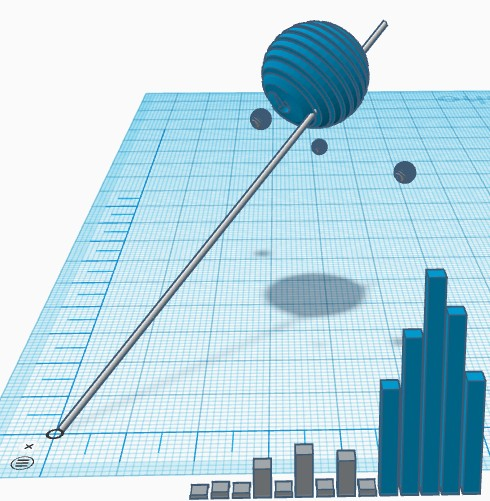
\includegraphics[scale=.8]{sections/images/consciousness_elliptical_orbit_system.jpg}
	\floatfoot{The subintervals decrease in speed as they move away from the peak of the wave.}%footnotemark}
	\end{figure}
	%\footnotetext{Fonte: note}

Yet another type of orbit is defined when the subintervals that orbit the peak of the wave maintain a constant average velocity regardless of the distance from the peak. This occurs because these subintervals are also part of the wave peak in blue, as shown in Figure \ref{fig:consciousness_circular_orbit_system}. Thus, because these subintervals remain in orbit within the 99.9\% subinterval of the wave, their velocities do not decrease. This 99.9\% of the wave is most easily visible part, therefore, the observed part of the galaxies, probably.
	\begin{figure}[H]
	\caption{Orbits of the subintervals inside the wave peak}
	\label{fig:consciousness_circular_orbit_system}
	\centering
	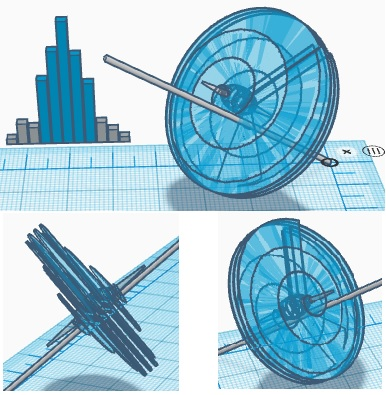
\includegraphics[scale=.9]{sections/images/consciousness_circular_orbit_system.jpg}
	\floatfoot{The subintervals maintain their speed as they move away from the peak of the wave.}%\footnotemark}
	\end{figure}
	%\footnotetext{Fonte: note}

For the distance of the subintervals in orbit, gravity exerts more of an orientation than an attraction. But since the motion is practically continuous in rarefied environments and this orientation is permanent, the orbits are formed and maintained by the increasing speed of these subintervals, which tends to pull them apart.

\subsubsubsection{Dark matter and dark energy}

\subsubsection{Antimatter}
When an interval tends to concentrate its samples toward the median, which is the probable direction according to the central limit theorem, it is called matter. Antimatter is the opposite, when an interval tends to concentrate its samples in the direction opposite to the median. 

The simplest way to visualize the probabilistic direction of samples of any wavelength is to look at the \textbf{probabilistic reference line}, as shown in Figure \ref{fig:consciousness_space_spiral_reference_line}. The greater the amount of sample in an interval, the greater will be its probabilistic tendency towards the population median.

In the Figure \ref{fig:consciousness_concentration_of_opposite_samples} two identical intervals are shown with their samples at opposite concentrations.
	\begin{figure}[H]
	\caption{Identical interval with its opposite sample concentrations}
	\label{fig:consciousness_concentration_of_opposite_samples}
	\centering
	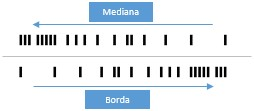
\includegraphics[scale=1.2]{sections/images/consciousness_concentration_of_opposite_samples.jpg}
	\floatfoot{Identical interval distributed in opposite ways.}%\footnotemark}
	\end{figure}
	%\footnotetext{Fonte: note}

Merging or summing the opposite intervals in Figure \ref{fig:consciousness_concentration_of_opposite_samples} would make them a symmetric interval, that is, it would not be in any direction.
The figure \ref{fig:consciousness_concentration_of_opposite_samples_within_range} shows one population with its samples concentrated toward the median and another with its samples concentrated toward the interval boundaries.
	\begin{figure}[H]
	\caption{Populations with their opposite sample concentrations}
	\label{fig:consciousness_concentration_of_opposite_samples_within_range}
	\centering
	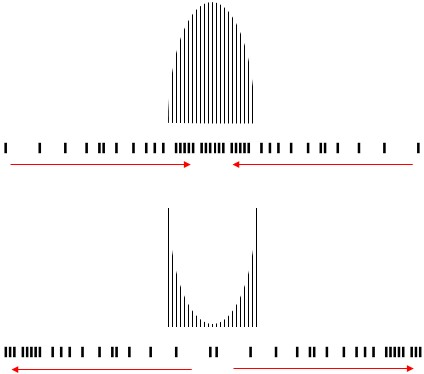
\includegraphics[scale=.7]{sections/images/consciousness_concentration_of_opposite_samples_within_range.jpg}
	\floatfoot{Populations distributed in opposite directions.}%\footnotemark}
	\end{figure}
	%\footnotetext{Fonte: note}

\subsubsection{Black Hole}
Black holes come from a probabilistic aspect present in any interval of the population. This aspect is the high probabilistic concentration of samples in smaller and smaller intervals of a wave. The peak will occupy a smaller and smaller proportional subinterval within the wave interval, even with an increasing sample concentration. These peaks are often found from the middle to the front of an interval or system (the core or peak of the system).

\subsubsection{Observer and life}
The wave intervals (wavelengths) that a subconsciousness (sublogic) is able to observe depend on the wavelengths of which the subconscious itself is composed. Among all the possibilities of intervals or wavelengths allowed by a population, the observer is in one of them. 

The ability to compare or distinguish the order of changes in a sequence of samples is the logical ability of an observer, the observer of time (past and present).The speed of this observation is given by the range that the observer is able to compare, that is, how quickly the observer is able to distinguish small changes (few samples - few logical moments) will make it realize that larger changes take longer (many samples - many logical moments).

The logical ability to make probabilistic prospections, within the logical limitations of the observer and based on the probability of distribution of the observed interval or subinterval, is the essence of thinking and, therefore, of life. These prospections are based on the probability of distribution of each interval (in the direction of the interval) and, therefore, are related to pattern detection and future probabilistic possibilities.

The ability to compare or distinguish logical waves (subsets or subconscious) is the ability that defines the subject [I - me]. The reasonableness of this definition depends on the proportionality of this ability to compare.

Life [IS NOT], like any other logic. Typically, the most notable life forms are multiplied by being on the probabilistic average of the interval between their peaks and valleys, however different they may be. Something very discrepant or different from the average pattern of the interval tends not to multiply and remain.

\subsubsubsection{Senses}
The cognitive part of a wave is not observed directly, but rather the outside - the consciousness, the whole or more commonly a part of that whole. This observation may include the rest of the wave that the cognitive part is part of, which is also external to the cognitive part, and so the cognitive part may be a nested subinterval of another. The cognitive part of the human subconscious is probably where the largest wave peak of the human subset is found. This is where the greatest intensity of change is observed. This great intensity of change is largely characterized by human thinking (observation and probabilistic prospecting of an interval) that tends toward infinity, as well as the essence of logic, the [NOT BEING].In other words, the cognitive part is the part that is closest to logic in its essence and also to its totality (consciousness).

The taking of samples by human beings, through the senses, modifies them and these ripples act as adjustments or configurations. Each sense observes the sample population independently, as distinct frequency channels. Thus, eyesight can be seeing objects very far away and ears hearing sounds that are very close. The senses are limited by the waves that constitute the observer and their maximum observation capacity is limited in the maximum depth of the nested intervals observed.

An important feature of the process of observing small intervals is that they can be observed with particles or waves. In particle observation, the observer follows an interval represented by an entangled pair, observing its consistent shape and movement in space. In the particle effect, the consistency of the shape and its movements are established by the entangled pair, since the jump occurs on one side of the pair at a time, guaranteeing stability in the changes. In the interval observed as a wave, the observer follows one of the parts that make up the entangled pair, observing its movements and jumps, since the jumps are frequent in small intervals.

It may not be possible to observe the wave effect without entangling its pair. The high frequency of this interval causes it to rapidly transit in an area around it, which may make it easier for it to reach a specific point in space, such as the human eye, that collapses its particle effect. This collapse can occur in a wider location (such as a wall or screen), and observe its wave effect with the collapse of many samples.
